\chapter{Introducción}
\label{chap1}
\ifpdf
  \graphicspath{{Chapter1/Chapter1Figs/PNG/}{Chapter1/Chapter1Figs/PDF/}{Chapter1/Chapter1Figs/}}
\else
  \graphicspath{{Chapter1/Chapter1Figs/EPS/}{Chapter1/Chapter1Figs/}}
\fi

\markboth{\hfill \thechapter. Introducción}{\hfill \thechapter. Introducción}

El impacto ambiental que provocan los residuos sólidos municipales ha sido objeto de atención especial en las últimas décadas. La eliminación de los residuos sólidos urbanos es una preocupación creciente en todo el mundo, sin importar el tamaño ni las características socio-económicas de una ciudad. Muchas ciudades se han visto obligadas a evaluar su programa de gestión de residuos sólidos y examinar su relación costo-efectividad en términos de recolección, transporte, tratamiento y eliminación \citep{Karadimas2007OptimalAlgorithm}.

En la Gestión de Residuos Sólidos (SWM, \textit{Solid Waste Management}) se estima que de la cantidad total de dinero destinado para su recogida, transporte y eliminación, aproximadamente el 60-80\% se gasta en la fase de Recolección de Residuos Sólidos (SWC, \textit{Solid Waste Collection}) \citep{Tavares2009OptimisationModelling,Dogan2003Report:Istanbul}. Por lo general, la fase de recolección en los países en desarrollo se basa en la experiencia práctica y en métodos intuitivos, dando lugar a prácticas ineficientes y costosas, que afectan tanto a la salud pública como al medio ambiente. Por ende, incluso una pequeña mejora en la operación de recogida puede dar lugar a un ahorro importante en el costo total, motivo por el cual muchos municipios se han esforzado en mejorar la gestión de la basura.

La Municipalidad de Asunción, de ahora en adelante MDA, cuenta con un conjunto de programas de trabajo anuales. En la Figura \ref{fig:porcentajePresupuesto} se puede observar que la mayor parte del presupuesto total de la municipalidad correspondiente al año 2017 fue destinado a los programas de acción. A su vez, dentro de estos programas de acción fue el servicio de calidad en recolección y limpieza el que se llevó la mayor parte y con una diferencia significativa sobre las demás, como se muestra en la Figura \ref{fig:programaAccion}.

\begin{figure}[H]
    \centering
    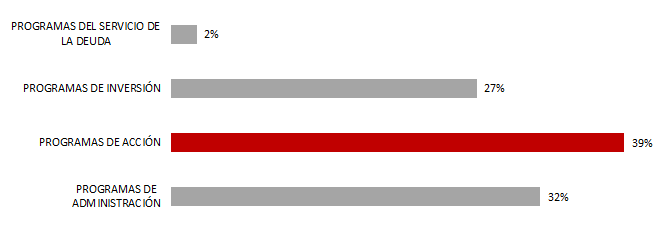
\includegraphics[width=14.5cm]{20181119_PresupuestoTotal2017.png}
    \caption{Representación porcentual del Presupuesto Total de la Municipalidad de Asunción discriminado por los programas para el año 2017. [Fuente: Portal de la Municipalidad de Asunción - Ejercicio Fiscal 2017]}
    \label{fig:porcentajePresupuesto}
\end{figure}

\begin{figure}[H]
    \centering
    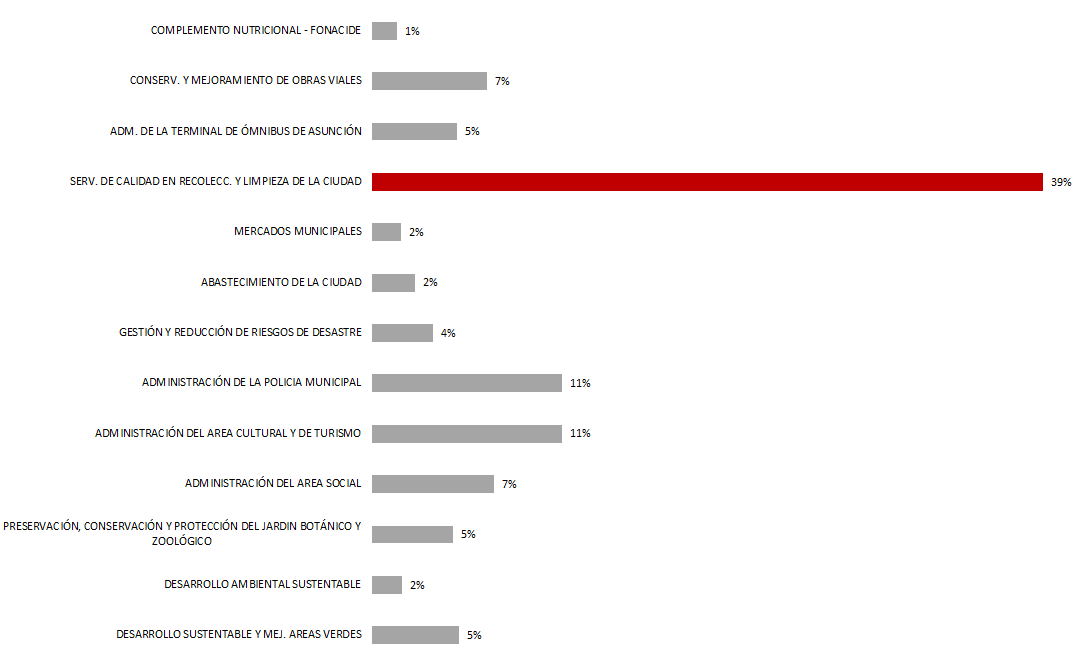
\includegraphics[width=15cm]{20181119_PresupuestoAccion2017.png}
    \caption{ Representación porcentual del Presupuesto correspondiente a los subprogramas del Programa de Acción correspondientes al año 2017. [Fuente: Portal de la Municipalidad de Asunción - Ejercicio Fiscal 2017]}
    \label{fig:programaAccion}
\end{figure}

\section{Antecedentes}

Cuando se habla de la problemática de la gestión de residuos sólidos, es sabido que existen numerosos estudios y trabajos científicos que se han realizado al respecto con el propósito de resolver usando objetivos económicos y ambientales como criterios para la toma de decisiones. Hasta la fecha, se siguen estudiando distintas técnicas que puedan permitir mejorar el proceso y como mencionan \citet{Tchobanoglous1993IntegratedIssues}, no existe un conjunto universal de reglas que puedan aplicarse a todas las situaciones.

% En la literatura, las soluciones al ruteo de la recolección de residuos sólidos urbanos se han planteado como distintos tipos de problemas, y están principalmente definidos en dos categorías: a) Problema de Enrutamiento de Vehículo Capacitado (CVRP, \textit{Capacitated Vehicle Routing Problem}), en donde se define una serie de nodos con demanda positiva cuyo objetivo es encontrar el mejor recorrido que cubra la totalidad de los nodos y; por otro lado, b) Problema de Enrutamiento de Arco Capacitado (CARP, \textit{Capacitated Arc Routing Problem}), en donde existe una serie de arcos predefinidos con demanda positiva o nula y el objetivo consiste en encontrar los mejores recorridos cubriendo todos los arcos requeridos \citep{Tirkolaee2018ATime}.

En la literatura, las soluciones al ruteo de la recolección de residuos sólidos urbanos se han planteado como distintos tipos de problemas, y están principalmente definidos en dos categorías \citep{Tirkolaee2018ATime}:

\begin{enumerate}[label=\alph*)]
    \item Problema de Enrutamiento de Vehículo Capacitado (CVRP, \textit{Capacitated Vehicle Routing Problem}), en donde se define una serie de nodos con demanda positiva cuyo objetivo es encontrar el mejor recorrido que cubra la totalidad de los nodos.
    \item Problema de Enrutamiento de Arco Capacitado (CARP, \textit{Capacitated Arc Routing Problem}), en donde existe una serie de arcos predefinidos con demanda positiva o nula y el objetivo consiste en encontrar los mejores recorridos cubriendo todos los arcos requeridos.
\end{enumerate}

% VRP CVRP VRPTW
En los enfoques que abordan el problema como un CVRP podemos citar a varios trabajos: \citet{Akhtar2017BacktrackingOptimization,Ombuki-Berman2007WASTEALGORITHMS,Kim2006WasteWindows,Billa2014GISOptimization,Karadimas2007OptimalAlgorithm}. En \citet{Akhtar2017BacktrackingOptimization} se desarrolló un Algoritmo de Búsqueda Hacia Atrás meta-heurístico (BSA, \textit{Backtracking Search Algorithm}) en un modelo CVRP con el concepto de contenedores inteligentes para encontrar las mejores soluciones de rutas de recolección. El estudio introduce el concepto de Umbral de Nivel de Residuos en contenedores (TWL, \textit{Threshold Waste Level}) para reducir el número de contenedores que deben ser vaciados al encontrar un rango óptimo de llenado, minimizando así la distancia, y consecuentemente reducir el combustible utilizado y las emisiones de gases.

\citet{Ombuki-Berman2007WASTEALGORITHMS} introduce el enfoque de un Algoritmo Genético multi-objetivo (GA, \textit{Genetic Algorithm}) para el enrutamiento de recolección de basura con ventanas de tiempo, minimizando el número total de vehículos y la distancia recorrida, atendiendo restricciones como capacidad de vehículo, ventanas de tiempo de parada y tiempos de almuerzo de conductores. El mayor potencial del algoritmo genético es que se puede utilizar en problemas prácticos de gran escala, buscando soluciones aproximadas en tiempo polinómico, en lugar de soluciones exactas que resultarían costosas para los de gran escala. Adoptó la definición del problema dado por \citet{Kim2006WasteWindows}, en donde se utilizó un algoritmo VRPTW de recolección de desechos basado en agrupación de nodos.

% TSP
Otros trabajos de la literatura tratan como un Problema del Vendedor Viajante (TSP, \textit{Travelling Sales Problem}), de hecho, el VRP surgió como una extensión del TSP para el caso en el que la capacidad de los vehículos que realizan la ruta sea limitada, siendo necesario realizar varios viajes \citep{CalvinoM2011CooperacionPanoramica}. En \citet{Billa2014GISOptimization} el enrutamiento óptimo se desarrolla con un método basado en el TSP y luego se integra con \textit{ArcInfo GIS} utilizando Programación Lineal (LP, \textit{Linear Programming}). Se reveló que las rutas óptimas pueden no ser necesariamente la distancia más corta desde el punto A al punto B, considerando la congestión del tráfico y la presencia de muchos semáforos en distancias cortas.

En \citet{Karadimas2007OptimalAlgorithm} se implementó un Sistema de Colonia de Hormigas (ACS, \textit{Ant Colony System}) para la identificación de rutas óptimas, que fue modelado como un TSP Asimétrico (ATSP, \textit{Asymmetric TSP}) para monitorear, simular, probar, y optimizar costos para diferentes escenarios de la WSM, donde un Sistema de Información Geográfica (GIS, \textit{Geographical Information System}) soporta la WSM usando parámetros como: la ubicación de cestos de basura, topología de red de carreteras, el tráfico relacionado y la densidad poblacional; además se consideran los horarios de recolección y las capacidades de los camiones.

En cuanto a la segunda categoría anteriormente mencionada, CARP, ha sido abordado por varios trabajos: \citet{Vecchi2016ACollection,Tirkolaee2018ATime,Braier2017AnArgentina}. En \citet{Vecchi2016ACollection} se presenta un enfoque secuencial para resolver el problema de optimización de la ruta de camiones recolectores. Se desarrolló un modelo para la solución del CARP, formulado como un Problema de Programación Lineal de Enteros Mixtos (MILP, \textit{Mixed Integer Linear Programming}), y luego se aplicó un algoritmo adaptado de Hierholzer para obtener la secuencia de los arcos. En \citet{Tirkolaee2018ATime} se presentó un interesane MILP para el problema de Enrutamiento de Arco Capacitado Periódico (PCARP, \textit{Periodic Capacitated Arc Routing Problem}) que tiene en cuenta los múltiples viajes, el tiempo de trabajo de los conductores y la tripulación para estudiar los efectos de la demanda incierta, para problemas de gran tamaño se aplicó un algoritmo híbrido basado en un algoritmo heurístico constructivo y un algoritmo de Recocido Simulado (SA, \textit{Simulated Annealing}).

% CPP, RPP, DRPP rural abierto.
Otro de los grandes problemas de arcos es el conocido como Problema del Cartero Rural (RPP, \textit{Rural Postman Problem}), que consiste en determinar el camino de mínima distancia que recorre solo algunos de los arcos del grafo y representa un problema \textit{NP-hard}, a no ser que el subgrafo formado por los arcos requeridos sea un grafo completamente conexo, en cuyo caso el RPP se reduce al Problema del Cartero Chino (CPP, \textit{Chinese Postman Problem}), para el cual se han definido algoritmos que lo resuelven en un tiempo polinómico \citep{CalvinoM2011CooperacionPanoramica}.

En \citet{Braier2017AnArgentina} se plantea un caso particular del RPP abierto Generalizado Dirigido (GDRPP, \textit{Generalized Directed Rural Postman Problem}). Desarrollaron un modelo de Programación de Enteros (IP, \textit{Integer Programming}) con un procedimiento de resolución basado en un algoritmo de mezcla de subtours y la adición dinámica de restricciones de eliminación de subtours. Este modelo sirvió de base para la implementación presentada en la siguiente sección.

% La herramienta ArcGIS Network Analytics (NA) es utilizada ampliamente en la búsqueda por minimizar la distancia y el tiempo de las rutas actuales de los camiones recolectores de residuos sólidos \citep{Kallel2016UsingTunisia, Malakahmad2014SolidMalaysia}. Existen además implementaciones comerciales similares a la solución que se propone, entre ellas se encuentran \textit{MapInfo Software}, \textit{RouteSmart}, \textit{Waste Route Software}, \textit{RouteViewPro}.
% % Agregar las implementacion libres.

% En este trabajo se propone el desarrollo de una herramienta, que optimice el camino seguido por los vehículos de recolección de basura de la ciudad de Asunción mediante técnicas de programación matemáticas, y consecuentemente, genere beneficios principalmente en los aspectos económicos y ambientales. Esta herramienta denominada de ahora en más \textit{TapeYty}, proveniente de dos palabras del idioma guaraní, \textit{Tape} que significa camino y \textit{Yty} que significa basura.

Varios modelos para la recolección y trasporte de los residuos sólidos han sido desarrollados basados en sistemas informáticos (\textit{software}) apropiados para la optimización de rutas. La herramienta ArcGIS Network Analytics (NA) es utilizada ampliamente en la búsqueda por minimizar la distancia y el tiempo de las rutas actuales de los camiones recolectores \citep{Kallel2016UsingTunisia,Malakahmad2014SolidMalaysia}. Existen además otras implementaciones comerciales, entre las que se encuentran \textit{MapInfo}, \textit{RouteSmart}, \textit{WasteRoute}, \textit{TransCAD}, \textit{RouteViewPro} mencionados en \citet{Kallel2016UsingTunisia} y \textit{Graphhopper} utilizado en \citet{Lozano2018SmartOptimization}.

Si bien los sistemas mencionados cumplen con el objetivo de optimizar los recorridos de vehículos, en su mayoría son de código cerrado y no se ajustan a los procedimientos específicos de una institución, resultando mucho más complejo y costoso extender sus funcionalidades. En este trabajo se propone el desarrollo de una herramienta sobre una arquitectura modular e interoperable, que optimice el camino a seguir por los vehículos de recolección de basura domiciliaria de la ciudad de Asunción mediante técnicas de programación matemáticas, y consecuentemente, genere beneficios principalmente en los aspectos económicos con la disminución de la distancia recorrida y en consecuencia el consumo de combustible; y ambientales con la disminución de la emisión de gases que dejan a su paso los camiones debido al menor tiempo de actividad \citep{Vu2018ParameterModel}. La herramienta denominada de ahora en adelante \textit{TapeYty}, proviene de dos palabras del idioma guaraní, \textit{Tape} que significa camino y \textit{Yty} que significa basura.

\section{Justificación}
 En la actualidad, los choferes de los vehículos recolectores de basura de la ciudad de Asunción trazan los caminos a seguir en base a su experiencia, razón por la cual es necesario optimizar el recorrido realizado para la recolección de residuos, reduciendo el costo y el tiempo de cada recorrido. Se propone desarrollar una aplicación que permita a la MDA gestionar de manera eficiente esos recorridos al poder actualizar el sentido de las calles, inhabilitar calles, agregar restricciones de giro o de contramano. La MDA podrá contar con una aplicación que garantice que todos los ciudadanos reciban el servicio de recolección domiciliaria.

El ingreso promedio de personas en ómnibus del transporte público y vehículos privados de los municipios aledaños, es alrededor de 1.320.000 a diario \citep{DiarioABCColor2016PorColor}, es así que no sólo los ciudadanos que residen en la ciudad de Asunción serán beneficiados con un servicio más eficiente, sino las miles de personas que ingresan diariamente a la ciudad, ya que al reducir el tiempo en tránsito del vehículo recolector se reducen los problemas de contaminación por los líquidos y gases que dejan a su paso.

Este proceso permitirá al personal encargado de la recolección de residuos agilizar su trabajo ya que pasarán menos tiempo en el vehículo recolector, mejorando así su calidad de vida.
 
Por todo lo expuesto, se considera plenamente justificada la investigación y propuesta de solución de este trabajo de fin de carrera, pues nos permitirá como ciudadanos retribuir en parte al Estado los beneficios y conocimientos que hemos adquirido a través de nuestra carrera en la Universidad.

\section{Objetivo General}
El objetivo general de este trabajo de investigación es el de proponer una solución que optimice el recorrido de los vehículos de recolección de basura domiciliaria de la Dirección Servicios Urbanos (DSU) de la MDA.

\section{Objetivos Específicos}

Los objetivos específicos que se han trazado en este trabajo son los siguientes:

\begin{enumerate}
    \item \textbf{Analizar} sobre técnicas de optimización para obtener el camino óptimo. 
    \item \textbf{Identificar} los factores que influyen en la recolección domiciliaria de la DSU.
    \item \textbf{Aplicar un modelo matemático} de optimización que mejor se ajuste a las reglas de negocio del caso de estudio.
    \item \textbf{Proponer y desarrollar una aplicación GIS} que permita configurar los parámetros de entrada del problema y despliegue la ruta óptima para cada zona de recolección.
    \item \textbf{Comparar} resultados de la aplicación desarrollada con los recorridos que actualmente son realizados, y de esta manera validar los resultados obtenidos.
\end{enumerate}


\section{Organización del Trabajo}

La organización del presente trabajo se completa de la siguiente manera:

\begin{itemize}
    \item En el \textbf{capítulo 2} se presentan los conceptos básicos que describen la gestión de residuos sólidos municipales y el caso de estudio, la ciudad de Asunción.
    \item En el \textbf{capítulo 3} se presentan conceptos básicos sobre Sistemas de Información Geográfica y bases de datos espaciales.
    \item En el \textbf{capítulo 4} se presentan las distintas técnicas de optimización.    
    \item En el \textbf{capítulo 5} se plantea de manera formal el problema que se intenta resolver. Se explican las formulaciones utilizadas, así como una explicación detallada de la implementación de la herramienta \textit{TapeYty}. 
    \item En el \textbf{capítulo 6} se visualizan y se discuten los resultados de la propuesta.
    \item En el \textbf{capítulo 7}, se finaliza el trabajo de investigación presentando las conclusiones generales, así como los aportes, aprendizajes y trabajos futuros continuando esta línea de investigación.
    % \item En el \textbf{capítulo ANEXOS}
\end{itemize}